% Options for packages loaded elsewhere
\PassOptionsToPackage{unicode}{hyperref}
\PassOptionsToPackage{hyphens}{url}
\PassOptionsToPackage{dvipsnames,svgnames,x11names}{xcolor}
%
\documentclass[
]{article}

\usepackage{amsmath,amssymb}
\usepackage{iftex}
\ifPDFTeX
  \usepackage[T1]{fontenc}
  \usepackage[utf8]{inputenc}
  \usepackage{textcomp} % provide euro and other symbols
\else % if luatex or xetex
  \usepackage{unicode-math}
  \defaultfontfeatures{Scale=MatchLowercase}
  \defaultfontfeatures[\rmfamily]{Ligatures=TeX,Scale=1}
\fi
\usepackage{lmodern}
\ifPDFTeX\else  
    % xetex/luatex font selection
    \setmainfont[]{Latin Modern Roman}
  \setmathfont[]{Latin Modern Math}
\fi
% Use upquote if available, for straight quotes in verbatim environments
\IfFileExists{upquote.sty}{\usepackage{upquote}}{}
\IfFileExists{microtype.sty}{% use microtype if available
  \usepackage[]{microtype}
  \UseMicrotypeSet[protrusion]{basicmath} % disable protrusion for tt fonts
}{}
\makeatletter
\@ifundefined{KOMAClassName}{% if non-KOMA class
  \IfFileExists{parskip.sty}{%
    \usepackage{parskip}
  }{% else
    \setlength{\parindent}{0pt}
    \setlength{\parskip}{6pt plus 2pt minus 1pt}}
}{% if KOMA class
  \KOMAoptions{parskip=half}}
\makeatother
\usepackage{xcolor}
\setlength{\emergencystretch}{3em} % prevent overfull lines
\setcounter{secnumdepth}{5}
% Make \paragraph and \subparagraph free-standing
\makeatletter
\ifx\paragraph\undefined\else
  \let\oldparagraph\paragraph
  \renewcommand{\paragraph}{
    \@ifstar
      \xxxParagraphStar
      \xxxParagraphNoStar
  }
  \newcommand{\xxxParagraphStar}[1]{\oldparagraph*{#1}\mbox{}}
  \newcommand{\xxxParagraphNoStar}[1]{\oldparagraph{#1}\mbox{}}
\fi
\ifx\subparagraph\undefined\else
  \let\oldsubparagraph\subparagraph
  \renewcommand{\subparagraph}{
    \@ifstar
      \xxxSubParagraphStar
      \xxxSubParagraphNoStar
  }
  \newcommand{\xxxSubParagraphStar}[1]{\oldsubparagraph*{#1}\mbox{}}
  \newcommand{\xxxSubParagraphNoStar}[1]{\oldsubparagraph{#1}\mbox{}}
\fi
\makeatother


\providecommand{\tightlist}{%
  \setlength{\itemsep}{0pt}\setlength{\parskip}{0pt}}\usepackage{longtable,booktabs,array}
\usepackage{calc} % for calculating minipage widths
% Correct order of tables after \paragraph or \subparagraph
\usepackage{etoolbox}
\makeatletter
\patchcmd\longtable{\par}{\if@noskipsec\mbox{}\fi\par}{}{}
\makeatother
% Allow footnotes in longtable head/foot
\IfFileExists{footnotehyper.sty}{\usepackage{footnotehyper}}{\usepackage{footnote}}
\makesavenoteenv{longtable}
\usepackage{graphicx}
\makeatletter
\def\maxwidth{\ifdim\Gin@nat@width>\linewidth\linewidth\else\Gin@nat@width\fi}
\def\maxheight{\ifdim\Gin@nat@height>\textheight\textheight\else\Gin@nat@height\fi}
\makeatother
% Scale images if necessary, so that they will not overflow the page
% margins by default, and it is still possible to overwrite the defaults
% using explicit options in \includegraphics[width, height, ...]{}
\setkeys{Gin}{width=\maxwidth,height=\maxheight,keepaspectratio}
% Set default figure placement to htbp
\makeatletter
\def\fps@figure{htbp}
\makeatother
% definitions for citeproc citations
\NewDocumentCommand\citeproctext{}{}
\NewDocumentCommand\citeproc{mm}{%
  \begingroup\def\citeproctext{#2}\cite{#1}\endgroup}
\makeatletter
 % allow citations to break across lines
 \let\@cite@ofmt\@firstofone
 % avoid brackets around text for \cite:
 \def\@biblabel#1{}
 \def\@cite#1#2{{#1\if@tempswa , #2\fi}}
\makeatother
\newlength{\cslhangindent}
\setlength{\cslhangindent}{1.5em}
\newlength{\csllabelwidth}
\setlength{\csllabelwidth}{3em}
\newenvironment{CSLReferences}[2] % #1 hanging-indent, #2 entry-spacing
 {\begin{list}{}{%
  \setlength{\itemindent}{0pt}
  \setlength{\leftmargin}{0pt}
  \setlength{\parsep}{0pt}
  % turn on hanging indent if param 1 is 1
  \ifodd #1
   \setlength{\leftmargin}{\cslhangindent}
   \setlength{\itemindent}{-1\cslhangindent}
  \fi
  % set entry spacing
  \setlength{\itemsep}{#2\baselineskip}}}
 {\end{list}}
\usepackage{calc}
\newcommand{\CSLBlock}[1]{\hfill\break\parbox[t]{\linewidth}{\strut\ignorespaces#1\strut}}
\newcommand{\CSLLeftMargin}[1]{\parbox[t]{\csllabelwidth}{\strut#1\strut}}
\newcommand{\CSLRightInline}[1]{\parbox[t]{\linewidth - \csllabelwidth}{\strut#1\strut}}
\newcommand{\CSLIndent}[1]{\hspace{\cslhangindent}#1}

\usepackage{arxiv}
\usepackage{orcidlink}
\usepackage{amsmath}
\usepackage[T1]{fontenc}
\makeatletter
\@ifpackageloaded{caption}{}{\usepackage{caption}}
\AtBeginDocument{%
\ifdefined\contentsname
  \renewcommand*\contentsname{Table of contents}
\else
  \newcommand\contentsname{Table of contents}
\fi
\ifdefined\listfigurename
  \renewcommand*\listfigurename{List of Figures}
\else
  \newcommand\listfigurename{List of Figures}
\fi
\ifdefined\listtablename
  \renewcommand*\listtablename{List of Tables}
\else
  \newcommand\listtablename{List of Tables}
\fi
\ifdefined\figurename
  \renewcommand*\figurename{Figure}
\else
  \newcommand\figurename{Figure}
\fi
\ifdefined\tablename
  \renewcommand*\tablename{Table}
\else
  \newcommand\tablename{Table}
\fi
}
\@ifpackageloaded{float}{}{\usepackage{float}}
\floatstyle{ruled}
\@ifundefined{c@chapter}{\newfloat{codelisting}{h}{lop}}{\newfloat{codelisting}{h}{lop}[chapter]}
\floatname{codelisting}{Listing}
\newcommand*\listoflistings{\listof{codelisting}{List of Listings}}
\makeatother
\makeatletter
\makeatother
\makeatletter
\@ifpackageloaded{caption}{}{\usepackage{caption}}
\@ifpackageloaded{subcaption}{}{\usepackage{subcaption}}
\makeatother

\ifLuaTeX
  \usepackage{selnolig}  % disable illegal ligatures
\fi
\usepackage{bookmark}

\IfFileExists{xurl.sty}{\usepackage{xurl}}{} % add URL line breaks if available
\urlstyle{same} % disable monospaced font for URLs
\hypersetup{
  pdftitle={thesis},
  pdfauthor={Dimitris Papachristopoulos},
  colorlinks=true,
  linkcolor={blue},
  filecolor={Maroon},
  citecolor={Blue},
  urlcolor={Blue},
  pdfcreator={LaTeX via pandoc}}


\newcommand{\runninghead}{A Preprint }
\title{thesis}
\def\asep{\\\\\\ } % default: all authors on same column
\author{\textbf{Dimitris Papachristopoulos}\\}
\date{}
\begin{document}
\maketitle

\renewcommand*\contentsname{Table of contents}
{
\hypersetup{linkcolor=}
\setcounter{tocdepth}{3}
\tableofcontents
}

\newpage{}

\section{Abstract}\label{abstract}

The Star Formation History (SFH) of a galaxy can offer many insights not
only for the evolution and the future of the galaxy, but also for the
evolution of the Universe. This is why there are various theoretical
models trying to describe the SFH of galaxies. One of those models is
the Delayed-Tau model, which approximates the Star Formation Rates (SFR)
of galaxies as a function with a rising SFR at the beginning, until it
reaches a peak at a time \(\tau\), unique for each galaxy, and then it
drops at an exponential rate.

Haslbauer, Kroupa, and Jerabkova (2023a) argues that the
Delayed-\(\tau\) model is opposed to the Lilly-Madau plot ((Madau and
Dickinson 2014)), which plots the observed SFR's of galaxies with the
corresponding redshifts (\(z\)) and calculates a cosmic SFR peak at
\(z\approx 2\). The way they calculated this inconsistency is by using
observatory data for SFR and Stellar Masses \footnote{They calculated
  the Stellar Masses by using a Mass to Light ratio of 0.6} from the
UNGC catalog (Karachentsev, Makarov, and Kaisina (2013), Karachentsev
and Kaisina (2013)) for calculating the parameters (the timescale
\(\tau\) and the normalization constant \(A_{del}\)) of the model. This
calculation for the galaxies of the Local Cosmological Volume (LCV),
allows the investigation of the SFR throughout the life each galaxy and
so we can find the expected time of peak of the SFR.

In this thesis project, we will try to calculate the same parameters, by
using a bigger sample size and the method Markov Chain Monte Carlo, to
examine if the inconsistencies of the model derive from the results of
the previous analysis, or if it is an intrinsic problem of the model

\textbf{Keywords:} Galaxies, Galaxy Evolution, Star Formation History
(SFH), Star Formation Rate (SFR), Delayed-\(\tau\), Local Cosmological
Volume, Lilly-Madau Plot, Redshift, Markov Chain Monte Carlo (MCMC).

\newpage{}

\section{Galaxy Morphology and Star-Forming
Regions}\label{galaxy-morphology-and-star-forming-regions}

\subsection{Galaxy Classification}\label{galaxy-classification}

\subsubsection{Hubble-de Vaucouleurs
Classification}\label{hubble-de-vaucouleurs-classification}

\subsubsection{Dwarf Galaxies}\label{dwarf-galaxies}

\subsection{Star-Forming Regions}\label{star-forming-regions}

\section{Star Formation History (SFH)}\label{star-formation-history-sfh}

The SFH of a galaxy describes the evolution of its star formation rate
over time. By selecting an appropriate model for SFH, we can analyze
stellar production, predict periods of active or quiescent star
formation, and determine when SFR stabilizes.

Understanding SFH models is crucial for interpreting internal and
external processes affecting galaxies and identifying conditions for
intense star formation in their early stages.

\subsection{Star Formation Rate}\label{star-formation-rate}

The star formation rate (SFR) is defined as the total gas mass of a
galaxy converted into stars over a specific time interval. It is
typically expressed in solar masses per year
(\(M_\odot \cdot \text{yr}^{-1}\)).

The SFR varies significantly over time, and its integration over time
provides the total stellar mass formed during the galaxy's history of
star formation. Specifically:

\begin{equation}\phantomsection\label{eq-sfr_int}{
\int_0^{t_{sf}} \text{SFR}(t)dt = \zeta M_*(t_{sf}),\ t_{sf}=\text{Time of Star Formation,} 
}\end{equation}

where \(\zeta\) accounts for mass loss during the Star Formation and is
approximately \(\zeta \approx 1.3\) (Kroupa et al. (2020)).

\subsubsection{Estimating SFR from
Spectra}\label{estimating-sfr-from-spectra}

SFR can be estimated using various photometric or spectroscopic methods
based on the luminosity of at least one spectral band or the intensity
of a spectral line. Different luminosities and intensities trace
distinct emission mechanisms, offering insights into a galaxy's
radiation sources. Below are common methods:

\footnote{\begin{itemize}
  \tightlist
  \item
    (Calzetti 2012), ({``{ASTR620 Galaxies} - {Fall} 2017''} n.d.)
  \end{itemize}}

\begin{itemize}
\item
  \textbf{Hα} \boldmath\(\alpha\) \textbf{Emission}: Young, hot, massive
  stars (O-type stars, \textasciitilde10 Myr, \textasciitilde20
  \(M_\odot\)) produce a number of ionizing photons, which they ionize
  the surrounding hydrogen rich gas. The hydorgen undergoes
  recombination cascades which produce Balmer emission lines of
  \(H\alpha\) (0.6563 \(\mu m\)) and \(H\beta\) (0.4861 \(\mu m\)). Dust
  can significantly affect observations.
\item
  \textbf{Far-Ultraviolet (FUV) Flux}: Mainly emitted by young, hot
  stars ( B-type stars, \textasciitilde100 Myr). Dust presence can also
  significantly affect observations.
\item
  \textbf{Infrared (IR) Flux}: The stars in a galaxy can heat up the
  dust in different ways, which then emits radiation in different parts
  of the IR spectrum. For example, young and massive, short-lived stars,
  emit UV radiation which then the heated dust emits in a wavelength of
  \(\approx 60 \mu m\), whereas dust heated by UV-faint old or low-mass
  stars will emit at \(\approx 100-150\mu m\). As a result, the total IR
  emission is age-agnostic and provides a more accurate approximation of
  the SFR because it accounts for contributions from both young and old
  stellar populations.
\item
  \textbf{Radio Continuum Emission}: Strongly correlated with IR. Its
  origin is complex, involving synchrotron radiation from relativistic
  electrons and thermal Bremsstrahlung from hot gas.
\item
  \textbf{X-Ray Emission}: In star-forming galaxies, X-rays arise from
  high-mass binary systems (neutron star or black hole with massive
  stellar companion) and hot gas from supernovae, correlating with SFR
  up to redshift \(z \sim 4\). X-rays are dust-insensitive, enabling
  accurate high-redshift observations.
\end{itemize}

SFR for different luminosities \(L_i\) can be calculated as:

\begin{equation}\phantomsection\label{eq-sfr-spectra}{
\text{SFR}_i = \mathcal{K}_i\times L_i
}\end{equation}

where \(\mathcal{K}_i\) is a constant specific to each \(L_i\) (\(i =\)
H\(\alpha\), IR, radio, FUV, X). In our analysis, we lack radio and
X-ray data.

Since the luminosities \(L_{\text{FUV}}\) and \(L_{\text{H}\alpha}\)
originate from young stars and are highly sensitive to dust, we either
directly observe stars unaffected by dust or use correction models to
account for dust absorption. It is crucial to ensure that these models
neither underestimate nor overestimate the luminosities by overlooking
or double-counting the same sources.

Additionally, because these luminosities are emitted by similar stellar
populations, we can reasonably expect the \(SFR_{\text{FUV}}\) and
\(SFR_{\text{H}\alpha}\) to be approximately equal. As shown in the data
from (Karachentsev and Kaisina 2013) and supported by (Kroupa et al.
2020), a suitable approach for estimating the total SFR from FUV and
H\(\alpha\) observations is to calculate their average:

\begin{equation}\phantomsection\label{eq-SFR_comb}{
SFR_{\text{FUV},H\alpha} = \text{mean}(SFR_{\text{FUV}}, SFR_{\text{H}\alpha}) 
}\end{equation}

where \(L_{\text{FUV}}\) and \(L_{\text{H}\alpha}\) are corrected for
dust attenuation.

\begin{figure}[H]

{\centering 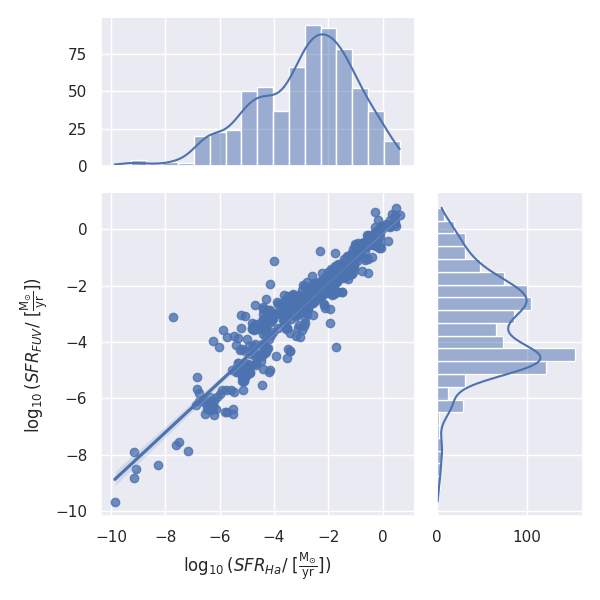
\includegraphics[width=5.20833in,height=\textheight]{figure/log_SFR_FUV_Ha.png}

}

\caption{Plot showing the linear relation
\(\log_{10}\text{SFR}_{FUV} = \log_{10}\text{SFR}_{H\alpha}\), as well
as their distrubutions}

\end{figure}%

According to (Madau and Dickinson 2014), this method often
underestimates the SFR, since different galaxy populations may
systematically follow distinct absorption mechanisms depending on their
characteristics.

Since \(SFR_{\text{FUV}}\), based on the uncorrected \(L_{FUV}\),
represents the emission from unobstructed stellar populations, and
\(SFR_{TIR}\) isaccounts for dust-reprocessed light, a more accurate way
to calculate the total SFR of a galaxy is:

\begin{equation}\phantomsection\label{eq-SFR_tot_madau}{
SFR_{\text{total}} = \mathcal{K}_{\text{FUV}} \cdot L_{\text{FUV}} + \mathcal{K}_{\text{IR}} \cdot L_{\text{IR}}
}\end{equation}

Following the same reasoning as the previous formula, the total SFR can
be expressed as:

\[
SFR_{\text{total}} = \text{mean}\left(\mathcal{K}_{\text{FUV}} \cdot L_{\text{FUV}}, \mathcal{K}_{\text{H}\alpha} \cdot L_{\text{H}\alpha}\right) + \mathcal{K}_{\text{IR}} \cdot L_{\text{IR}} \\
= SFR_{\text{FUV},H\alpha}+ SFR_{\text{IR}}
\]

where \(L_{\text{FUV}}\) and \(L_{\text{H}\alpha}\) are not corrected
for dust absorption. However, since we do not have enough galaxies with
both traces, we will use a different method of calculating the total
SFR, which we will discuss later.

\subsection{Main Sequence Galaxies}\label{main-sequence-galaxies}

The SFR and stellar mass of a galaxy are tightly correlated by the
relationship:

\[
\log(\text{SFR}) = \alpha \log(M_*)+\beta
\]

where \(\alpha(t)\) and \(\beta(t)\) depend on time and redshift \(z\)
(Speagle et al. (2014)):

\subsubsection{Star Formation History
Models}\label{star-formation-history-models}

Parameterized SFH models are commonly used, offering simplicity through
a few parameters (Carnall et al. (2019)):

\begin{itemize}
\tightlist
\item
  \textbf{Exponential Decline (Tau Model):} The star formation rate
  (SFR) decreases exponentially over time, following the equation:
\end{itemize}

\[
  \text{SFR}(t) \propto e^{-t_{\text{sf}}/\tau}
\]

where \(\tau\) is the timescale, \(t_{\text{sf}} = t - T_0\) is the star
formation time, \(t\) is the age of the Universe, and \(T_0\) is the
time when star formation began.

\begin{itemize}
\tightlist
\item
  \textbf{Delayed Exponential (Delayed Tau Model):} This model provides
  a more complex representation where the SFR initially increases,
  reaches a peak, and then declines exponentially over time. The
  equation for this model is:
\end{itemize}

\[
  \text{SFR}(t) \propto t_{\text{sf}} e^{-t_{\text{sf}}/\tau}
\]

This accounts for an initial growth phase followed by a decline. In this
case, \(\tau\) represents the time it takes for the galaxy to reach
\(\text{SFR}_{\text{max}}\).

\begin{itemize}
\tightlist
\item
  \textbf{Log-Normal Distribution Model:} The SFR follows a normalized
  log-normal distribution, which can accurately model the star formation
  rate density (\(\text{SFRD} = \text{SFR}/M_*\)) in individual
  galaxies. The general form of the equation is:
\end{itemize}

\[
  \text{SFR}(t) \propto \frac{1}{\tau} \exp\left(-\frac{(\ln(t) - T_0)^2}{2\tau^2}\right)
\]

where \(\tau\) and \(T_0\) are free parameters of the distribution that
lack physical significance, as the SFR does not necessarily peak at
\(t = e^{T_0}\).

\begin{itemize}
\tightlist
\item
  \textbf{Double Power Law:} This model describes a scenario where the
  SFR rises and then falls sharply, useful for modeling galaxies
  experiencing rapid changes in star formation. The equation is:
\end{itemize}

\[
  \text{SFR}(t) \propto \left[\left(\frac{t}{\tau}\right)^\alpha + \left(\frac{t}{\tau}\right)^\beta\right]^{-1}
\]

where \(\tau\) is the timescale and \(\alpha\), \(\beta\) are exponents
that govern the rise and fall of the SFR.

\begin{figure}[H]

{\centering 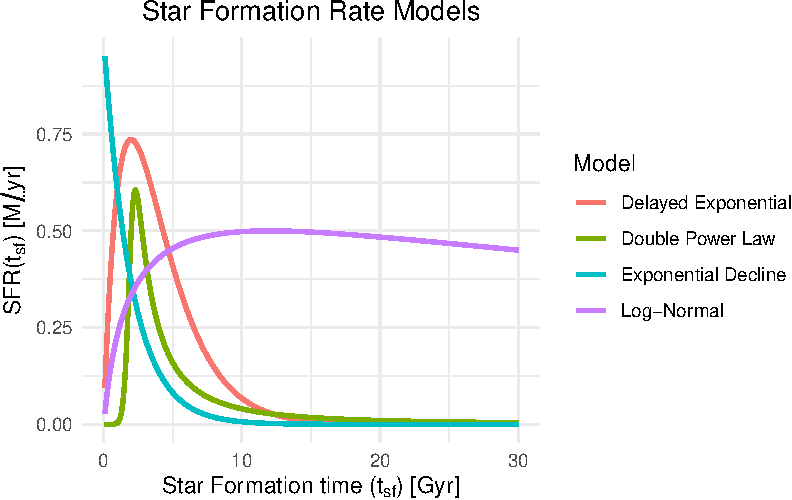
\includegraphics{thesis_files/figure-pdf/unnamed-chunk-2-1.pdf}

}

\caption{Star Formation Rate over the time of star formation, for
different parametric models}

\end{figure}%

Additionally, there are non-parametric models, which do not follow a
specific functional form to describe the star formation of a galaxy.
These models are more flexible in adapting to galaxies with more complex
star formation patterns.

\subsection{\texorpdfstring{Delayed-\(τ\)
Model}{Delayed-τ Model}}\label{delayed-ux3c4-model}

The delayed \(τ\) model is widely used for describing an initial
starburst followed by a gradual decline in SFR. This places galaxies on
the main sequence. It is particularly effective for massive galaxies
(Haslbauer, Kroupa, and Jerabkova (2023b)). However, it assumes smooth
SFR evolution and may overestimate peak SFR in high-redshift galaxies.

Using the delayed τ model, we compute \(\tau\), \(t_{\text{sf}}\), and
normalization constant \(A_{\text{del}}\) with:

\begin{equation}\phantomsection\label{eq-delayed-current}{
\text{SFR}_0 = \text{SFR}(t_{sf}) = A_{del}\frac{t_{sf}}{\tau^2}e^{-t_{sf}/\tau}
}\end{equation}

where \(\text{SFR}_0\) is given in the catalogs.

\section{Lilly-Madau Plot}\label{lilly-madau-plot}

The Lilly-Madau plot is one of the most important plots in the field of
galaxy evolution. It describes how the SFRD of the universe evolved over
time, with observational data. to figure out

\subsection{Redshift and lookback
time}\label{redshift-and-lookback-time}

According to Hubble--Lemaître law, all the galaxies are moving away from
each other, at a speed proportional to their distance, due to the
expansion of the universe.

\(V = H_0\times d\), where \(H_0 \approx 69.8 \text{ km/s/Mpc}\) is the
Hubble constant and \(d\) is the distance between the two
galaxies.\footnote{We also have non-Hubble motions
  \(V = H_0\times d + V_0\), where \(V_0\) is the peculiar velocity and
  it could, for example, be due to galaxy cluster dynamics. For the
  current explanation we are going to ignore it. This way the radial
  velocity \(v\) is equal to \(V\)}

Since we have galaxies with relative motions emitting light waves, we
can observe the Doppler effect. Specifically, since the galaxies are
moving away from each other, and thus from us also, we observe radiation
with longer wavelenghts.

\emph{Redshift} (\(z\)) is the doppler shift resulting from radial
motion:

\[
z = \frac{\lambda_{observed}}{\lambda_{emitted}}-1
\]

In special relativity, \(z\) is related to radial velocity \(v\) by
(Hogg, n.d.)

\begin{equation}\phantomsection\label{eq-z-rel}{
1+z = \sqrt{\frac{1+v/c}{1-v/c}}
}\end{equation} For small \(v/c\) we can rewrite
Equation~\ref{eq-z-rel}, as:

\[
z \approx \frac{V}{c} = \frac{H_0\times d}{c}
\]

But, because light takes time to cover the distance \(d\) between two
galaxies, when the light finally reaches as, we will see the observed
galaxy, as it was when the light was emitted, and not how it is at this
moment. If we substitute time that it took the light to reach us over
the distance, then we arrive at the relation (Longair 1998):

\[
t_\text{emitted} \propto z^{-3/2}
\]

\emph{The lookback time} is the difference between the current age of
the Universe and the age of the Universe when the light was emitted

\[
t_L = T_0-t_\text{emitted}
\]

\section{Lilly-Madau Plot}\label{lilly-madau-plot-1}

\section{\texorpdfstring{Delayed-\(\tau\)
model}{Delayed-\textbackslash tau model}}\label{delayed-tau-model}

\section{Computational Methods}\label{computational-methods}

\subsection{Newton-Raphson}\label{newton-raphson}

\subsection{Markov Chain Monte Carlo}\label{markov-chain-monte-carlo}

\section{Prepering the Catalogs}\label{prepering-the-catalogs}

UNGC HECATE join etc\ldots{}

\subsection{Catalog Completeness}\label{catalog-completeness}

\subsection{Comparing the Catalogs}\label{comparing-the-catalogs}

\subsection{The ``special'' case of the Star Formation
Rates}\label{the-special-case-of-the-star-formation-rates}

\section{Calculating the parameters}\label{calculating-the-parameters}

\subsection{According to pre-existing
bibliography}\label{according-to-pre-existing-bibliography}

\subsubsection{Problems with the method}\label{problems-with-the-method}

\subsection*{MCMC}\label{mcmc}
\addcontentsline{toc}{subsection}{MCMC}

\phantomsection\label{refs}
\begin{CSLReferences}{1}{0}
\bibitem[\citeproctext]{ref-ASTR620GalaxiesFall}
{``{ASTR620 Galaxies} - {Fall} 2017.''} n.d. Accessed October 27, 2024.
\url{https://www.astro.umd.edu/~richard/ASTRO620/index_fall2017.html}.

\bibitem[\citeproctext]{ref-calzettiStarFormationRate2012}
Calzetti, Daniela. 2012. {``Star {Formation Rate Indicators}.''} August
15, 2012. \url{http://arxiv.org/abs/1208.2997}.

\bibitem[\citeproctext]{ref-carnallHowMeasureGalaxy2019a}
Carnall, Adam C., Joel Leja, Benjamin D. Johnson, Ross J. McLure, James
S. Dunlop, and Charlie Conroy. 2019. {``How to {Measure Galaxy Star
Formation Histories}. {I}. {Parametric Models}.''} \emph{The
Astrophysical Journal} 873 (1): 44.
\url{https://doi.org/10.3847/1538-4357/ab04a2}.

\bibitem[\citeproctext]{ref-haslbauerCosmologicalStarFormation2023}
Haslbauer, Moritz, Pavel Kroupa, and Tereza Jerabkova. 2023b. {``The
Cosmological Star Formation History from the {Local Cosmological Volume}
of Galaxies and Constraints on the Matter Homogeneity.''} \emph{Monthly
Notices of the Royal Astronomical Society} 524 (3): 3252--62.
\url{https://doi.org/10.1093/mnras/stad1986}.

\bibitem[\citeproctext]{ref-haslbauer2023}
---------. 2023a. {``The Cosmological Star Formation History from the
Local Cosmological Volume of Galaxies and Constraints on the Matter
Homogeneity.''} \emph{Monthly Notices of the Royal Astronomical Society}
524 (3): 3252--62. \url{https://doi.org/10.1093/mnras/stad1986}.

\bibitem[\citeproctext]{ref-hoggDistanceMeasuresCosmology2000}
Hogg, David W. n.d. {``Distance Measures in Cosmology.''}
\url{https://doi.org/10.48550/arXiv.astro-ph/9905116}.

\bibitem[\citeproctext]{ref-karachentsevSTARFORMATIONPROPERTIES2013}
Karachentsev, Igor D., and Elena I. Kaisina. 2013. {``{STAR FORMATION
PROPERTIES IN THE LOCAL VOLUME GALAXIES VIA Hα AND FAR-ULTRAVIOLET
FLUXES}.''} \emph{The Astronomical Journal} 146 (3): 46.
\url{https://doi.org/10.1088/0004-6256/146/3/46}.

\bibitem[\citeproctext]{ref-karachentsev2013}
Karachentsev, Igor D., Dmitry I. Makarov, and Elena I. Kaisina. 2013.
{``UPDATED NEARBY GALAXY CATALOG.''} \emph{The Astronomical Journal} 145
(4): 101. \url{https://doi.org/10.1088/0004-6256/145/4/101}.

\bibitem[\citeproctext]{ref-kroupaConstraintsStarFormation2020}
Kroupa, P, M Haslbauer, I Banik, S T Nagesh, and J Pflamm-Altenburg.
2020. {``Constraints on the Star Formation Histories of Galaxies in the
{Local Cosmological Volume}.''} \emph{Monthly Notices of the Royal
Astronomical Society} 497 (1): 37--43.
\url{https://doi.org/10.1093/mnras/staa1851}.

\bibitem[\citeproctext]{ref-longairGalaxyFormation1998}
Longair, Malcolm S. 1998. \emph{Galaxy Formation}. Springer Science \&
Business Media.

\bibitem[\citeproctext]{ref-madau2014}
Madau, Piero, and Mark Dickinson. 2014. {``Cosmic Star Formation
History.''} \emph{Annual Review of Astronomy and Astrophysics} 52 (1):
415--86. \url{https://doi.org/10.1146/annurev-astro-081811-125615}.

\bibitem[\citeproctext]{ref-speagleHighlyConsistentFramework2014}
Speagle, Joshua S., Charles L. Steinhardt, Peter L. Capak, and John D.
Silverman. 2014. {``A {Highly Consistent Framework} for the {Evolution}
of the {Star-Forming} "{Main Sequence}" from z\textasciitilde0-6.''}
\emph{The Astrophysical Journal Supplement Series} 214 (2): 15.
\url{https://doi.org/10.1088/0067-0049/214/2/15}.

\end{CSLReferences}




\end{document}
